% Part 1 — Medium (set01)

\begin{problem}[The transformed uniform distribution]
Let $X$ be discrete uniform on the first $n$ positive odd integers
\[
1,3,5,\ldots,2n-1.
\]
For comparison, let $U$ be discrete uniform on $\{1,2,\ldots,n\}$, with
\[
E(U)=\frac{n+1}{2},\qquad \mathrm{Var}(U)=\frac{n^2-1}{12}.
\]
The key idea is to recognise the odd integers as a linear transformation of the simpler variable $U$.
\begin{enumerate}[label=\textbf{(\roman*)}]
  \item Give $P(X=x)$ for outcomes in the sample space.
  \item Write $X$ as a linear function of $U$ and find $E(X)$.
  \item Find $\mathrm{Var}(X)$ in terms of $n$.
  \item Let $S=X_{1}+X_{2}$ be the sum of two independent draws. Find $E(S)$, $\mathrm{Var}(S)$, and $P(S\text{ is maximal})$.
\end{enumerate}
\end{problem}

\begin{hint}
\begin{itemize}[leftmargin=*]
  \item Odd integers are $2k-1$: relate $X$ to $U$ by $X=2U-1$.
  \item Use $\mathrm{Var}(aU+b)=a^{2}\mathrm{Var}(U)$.
  \item Maximal $S$ arises only when both draws equal $2n-1$.
\end{itemize}
\end{hint}

\begin{solution}
\textbf{(i)} $n$ equally likely values: $P(X=x)=\frac{1}{n}$ for each allowed $x$.

\textbf{(ii)} $X=2U-1$, so $E(X)=2E(U)-1=n$.

\textbf{(iii)} $\mathrm{Var}(X)=\mathrm{Var}(2U-1)=4\mathrm{Var}(U)=\frac{n^{2}-1}{3}$.

\textbf{(iv)} Since $X_1$ and $X_2$ are independent copies of $X$,
\[
E(S)=E(X_1)+E(X_2)=n+n=2n.
\]
Independence also lets us add variances:
\[
\mathrm{Var}(S)=\mathrm{Var}(X_1)+\mathrm{Var}(X_2)=\frac{2(n^2-1)}{3}.
\]
The largest possible sum is
\[
(2n-1)+(2n-1)=4n-2,
\]
and this occurs only when both draws equal $2n-1$. Each has probability $1/n$, so
\[
P(S\text{ is maximal})=\frac1n\cdot\frac1n=\frac{1}{n^2}.
\]
\end{solution}

\begin{takeaways}
\item Affine maps $U\mapsto 2U-1$ avoid summing long arithmetic lists.
\item Variance scales with the square of the multiplier on $U$.
\item Sums of i.i.d.\ discrete uniforms have a peaked distribution---extreme totals are rare ($1/n^{2}$ here).
\end{takeaways}

\begin{problem}[The asymmetric triangular distribution]
A continuous random variable $X$ has a triangular-shaped pdf which rises linearly from $0$ to a peak at $x=1$, then falls linearly to $0$ at $x=3$:
\[
f(x)=\begin{cases}
cx & 0\le x\le 1\\
c\bigl(\frac{3-x}{2}\bigr) & 1< x\le 3\\
0 & \text{otherwise.}
\end{cases}
\]
\begin{enumerate}[label=\textbf{(\roman*)}]
  \item Find $c$, sketch $y=f(x)$, and check $f(x)\ge 0$.
  \item Show total area is $1$ by geometry and by integration.
  \item Find the cdf $F(x)$.
  \item Find the lower quartile $Q_{1}$ and median $Q_{2}$.
\end{enumerate}

\begin{center}\small
\begin{tikzpicture}[x=1.25cm,y=6.5cm]
  \def\cval{0.666666} % c = 2/3
  \fill[blue!60!gray, opacity=0.28]
    (0,0) -- (1,\cval) -- (3,0) -- cycle;
  \draw[thick, blue!75!black] (0,0) -- (1,\cval) -- (3,0) -- (0,0);
  \draw[->] (-0.3,0) -- (3.35,0) node[right, font=\small] {$x$};
  \draw[->] (0,-0.05) -- (0,0.78) node[above, font=\small] {$f(x)$};

  \foreach \xb/\lbl in {0/$0$,1/$1$,3/$3$}{
    \draw (\xb,0) -- ++(0,-0.035) node[below, font=\scriptsize] {\lbl};
  }
  \node[right, font=\scriptsize] at (1,\cval) {peak $c=\tfrac23$};
\end{tikzpicture}\\[0.35em]

\noindent\footnotesize\textit{Asymmetric triangle pdf on $[0,3]$ with peak at $x=1$ (area $=1$).}
\end{center}

\end{problem}

\begin{hint}
\begin{itemize}[leftmargin=*]
  \item Triangular area on $[0,3]$ with peak at $x=1$.
  \item Split $\int_{0}^{1}$ and $\int_{1}^{3}$.
  \item Compare target probabilities to $F(1)=\frac{1}{3}$.
  \item Quadratic on the second branch: keep roots in $(1,3]$.
\end{itemize}
\end{hint}

\begin{solution}
\textbf{(i)} Area $\tfrac12\cdot 3\cdot f(1)=\tfrac12\cdot 3\cdot c=1\Rightarrow c=\frac{2}{3}$. Then $f(x)=\frac{2}{3}x$ on $[0,1]$ and $\frac{1}{3}(3-x)$ on $(1,3]$ --- nonnegative on $[0,3]$.

\textbf{(ii)} Geometrically, the graph is a triangle with base length $3$ and height $c=\frac23$, so its area is
\[
\frac12\cdot3\cdot\frac23=1.
\]
By integration,
\[
\int_0^1 \frac23x\,dx+\int_1^3 \frac13(3-x)\,dx
=\frac13+\frac23=1.
\]
Both methods confirm that $f$ has total area $1$.

\textbf{(iii)} $F(x)=0$ for $x<0$; for $0\le x\le 1$, $F(x)=\frac{x^{2}}{3}$; for $1<x\le 3$, $F(x)=\frac{1}{3}+\int_{1}^{x}\frac{1}{3}(3-t)\,dt=x-\frac{x^{2}}{6}-\frac12$; for $x>3$, $F=1$.

\textbf{(iv)} $Q_{1}$ solves $\frac{x^{2}}{3}=0{.}25$, so $Q_{1}=\frac{\sqrt{3}}{2}$. For $Q_{2}$, $x-\frac{x^{2}}{6}-\frac12=\frac12$ yields $Q_{2}=3-\sqrt{3}$.
\end{solution}

\begin{takeaways}
\item Piecewise pdfs splice cdfs continuously at joins.
\item Check $F(1)$ before selecting which cdf branch solves $F=q$.
\item Respect domain constraints when rejecting quadratic roots.
\end{takeaways}

\begin{problem}[The variance identity and mean squared error]
Let $X$ have pdf $f(x)$ and mean $\mu$. This problem proves two useful identities: the computational formula for variance and the decomposition of mean squared error. The final parts apply the identities to a symmetric density.
\begin{enumerate}[label=\textbf{(\roman*)}]
  \item Prove $\displaystyle\int_{-\infty}^{\infty}(x-\mu)^{2}f(x)\,dx=\int_{-\infty}^{\infty}x^{2}f(x)\,dx-\mu^{2}$.
  \item Show $\displaystyle\int_{-\infty}^{\infty}(x-c)^{2}f(x)\,dx=\mathrm{Var}(X)+(\mu-c)^{2}$.
  \item For $f(x)=\frac{3}{4}(1-x^{2})$ on $[-1,1]$, compute $\mathrm{Var}(X)$.
  \item Minimize $E[(X-c)^{2}]$ over constants $c$ for this $f$.
\end{enumerate}
\end{problem}

\begin{hint}
\begin{itemize}[leftmargin=*]
  \item Expand $(x-\mu)^{2}$ and integrate termwise.
  \item Write $(x-c)=(x-\mu)+(\mu-c)$ and expand the square---the cross-term integrates to $0$.
  \item $f$ is even on $[-1,1]$, hence $\mu=0$.
  \item The expression in (ii) is minimized when $(\mu-c)^{2}=0$.
\end{itemize}
\end{hint}

\begin{solution}
\textbf{(i)} Expand the square inside the integral:
\[
\int_{-\infty}^{\infty}(x-\mu)^2f(x)\,dx
=\int (x^2-2\mu x+\mu^2)f(x)\,dx.
\]
Using $\int f(x)\,dx=1$ and $\int xf(x)\,dx=\mu$, this becomes
\[
\int x^2f(x)\,dx-2\mu^2+\mu^2
=\int x^2f(x)\,dx-\mu^2.
\]

\textbf{(ii)} Write
\[
x-c=(x-\mu)+(\mu-c).
\]
After squaring and integrating,
\[
E[(X-c)^2]=E[(X-\mu)^2]+2(\mu-c)E(X-\mu)+(\mu-c)^2.
\]
The middle term is $0$ because $E(X-\mu)=0$, so
\[
E[(X-c)^2]=\mathrm{Var}(X)+(\mu-c)^2.
\]

\textbf{(iii)} Symmetry yields $\mu=0$. Thus $\mathrm{Var}(X)=E(X^{2})=\frac{3}{4}\int_{-1}^{1}x^{2}(1-x^{2})\,dx=\frac{1}{5}$.

\textbf{(iv)} Unique minimizer $c=\mu=0$, with minimum $\mathrm{Var}(X)=\frac{1}{5}$.
\end{solution}

\begin{takeaways}
\item Computational variance $E(X^{2})-\mu^{2}$ comes straight from expanding squares.
\item MSE decomposition shows the mean minimizes expected squared error.
\item Even pdf on symmetric support $\Rightarrow \mu=0$.
\end{takeaways}

\begin{problem}[Evaluating clinical trial efficacy]
A drug has a baseline helpful-response rate of $70\%$ under the usual delivery method. We use $p=0{.}7$ as the reference probability and compare trial results against the binomial model using normal approximations.
\begin{enumerate}[label=\textbf{(\roman*)}]
  \item Team A: $n=50$, $45$ responders. Assuming $X\sim B(50,\,0{.}70)$ under the null/reference, compute the approximate $z$-score for observing at least $45$ successes using the normal approximation with \emph{continuity correction}.

  \item Team B expects exactly $80\%$ successes in $n$ patients $(0{.}8n\in\mathbb{Z})$. Ignoring corrections, determine the smallest $n$ whose uncorrected $z$-score (relative to baseline $p=0{.}7$) strictly exceeds Team A's \emph{uncorrected} $z$-score for $45/50$.
\end{enumerate}
\end{problem}

\begin{hint}
\begin{itemize}[leftmargin=*]
  \item For $\ge 45$, use boundary $44.5$ versus $N(np,\,npq)$.
  \item Compare $z_{B}(n)=(0{.}8n-0{.}7n)/\sqrt{0{.}21n}$ with $z_{A}=(45-35)/\sqrt{10{.}5}$, then enforce divisibility constraints.
\end{itemize}
\end{hint}

\begin{solution}
\textbf{(i)} $\mu=35$, $\sigma^{2}=10{.}5$. With correction, $z=\frac{44{.}5-35}{\sqrt{10{.}5}}=\frac{9{.}5}{\sqrt{10{.}5}}\approx 2{.}93$.

\textbf{(ii)} For comparison, Team A's uncorrected score is
\[
z_A=\frac{45-35}{\sqrt{10{.}5}}=\frac{10}{\sqrt{10{.}5}}.
\]
If Team B has exactly $0{.}8n$ responders, its uncorrected score relative to the baseline mean $0{.}7n$ is
\[
z_B(n)=\frac{0{.}8n-0{.}7n}{\sqrt{0{.}7(0{.}3)n}}
=\frac{0{.}1n}{\sqrt{0{.}21n}}
=\sqrt{\frac{n}{21}}.
\]
We require $z_B(n)>z_A$, so
\[
\sqrt{\frac{n}{21}}>\frac{10}{\sqrt{10{.}5}}
\quad\Longrightarrow\quad n>200.
\]
Also $0{.}8n$ must be an integer, so $n$ must be a multiple of $5$. The smallest valid value greater than $200$ is $\boxed{205}$.
\end{solution}

\begin{takeaways}
\item Continuity corrections matter when $n$ is modest.
\item Evidence strength depends both on proportion and effective sample size.
\item Algebraic isolation of $\sqrt{n}$ simplifies comparisons cleanly.
\end{takeaways}

\begin{problem}[The musical fundraiser]
At a school musical fundraiser, attendees spent different amounts on tickets, snacks, and small donations. Instead of recording every exact amount, the organisers grouped the spending into \$10 intervals. In the table below, each \textbf{class} is a spending interval, the \textbf{centre} $x_i$ is the midpoint used to represent everyone in that interval, and the \textbf{frequency} $f_i$ is the number of attendees in that interval.

Grouped spending (\$):

\begin{center}
\small
\begin{tabular}{|l|c|c|c|c|c|}
\hline
class & $0\le x<10$ & $10\le x<20$ & $20\le x<30$ & $30\le x<40$ & $40\le x<50$ \\
centre $x_{i}$ & $5$ & $15$ & $25$ & $35$ & $45$ \\
frequency $f_{i}$ & $30$ & $a$ & $45$ & $b$ & $15$ \\
\hline
\end{tabular}
\end{center}

There are $\sum f_{i}=150$ attendees with mean \$21 estimated from class centres.
\begin{enumerate}[label=\textbf{(\roman*)}]
  \item Find $a$ and $b$.
  \item Find $\mathrm{Var}(X)$ using class centres, and estimate the median amount spent using cumulative frequencies.
  \item Assuming uniformity within classes, approximate $P(X>28)$.
  \item For profit $P=0{.}6X-5$, find $E(P)$ and $\sigma(P)$.
\end{enumerate}
\end{problem}

\begin{hint}
\begin{itemize}[leftmargin=*]
  \item Use $\sum f=150$ and $\frac{\sum f x}{\sum f}=21$.
  \item $\mathrm{Var}(X)=E(X^{2})-\mu^{2}$ with discrete weights $f_{i}/150$.
  \item From $\$28$ upward, accumulate partial class $[20{,}30)$.
  \item $\mathrm{Var}(aX+b)=a^{2}\mathrm{Var}(X)$.
\end{itemize}
\end{hint}

\begin{solution}
\textbf{(i)} The total frequency gives
\[
30+a+45+b+15=150\quad\Rightarrow\quad a+b=60.
\]
The mean condition gives $\sum f_ix_i=150(21)=3150$. The known contributions are
\[
30(5)+45(25)+15(45)=1950,
\]
so
\[
15a+35b=3150-1950=1200.
\]
Solving the simultaneous equations gives $\boxed{a=45,\ b=15}$.

\textbf{(ii)} Using the class centres,
\[
E(X^2)=\frac{\sum f_ix_i^2}{150}=585.
\]
Since $\mu=21$,
\[
\mathrm{Var}(X)=E(X^2)-\mu^2=585-21^2=\boxed{144}.
\]
For the median, the cumulative frequencies are $30,75,120,135,150$. The middle position lies at the boundary between the second and third classes, so the median is estimated as $\boxed{\$20}$.

\textbf{(iii)} Within the $20\le x<30$ class, the portion above $28$ is the interval from $28$ to $30$, which is $\frac{2}{10}$ of the class width. Assuming uniformity, this contributes
\[
\frac{2}{10}\cdot45=9
\]
attendees. All attendees in the $30$--$40$ and $40$--$50$ classes also count, giving $9+15+15=39$. Hence
\[
P(X>28)\approx\frac{39}{150}=\boxed{0{.}26}.
\]

\textbf{(iv)} $E(P)=0{.}6(21)-5=7{.}60$; $\mathrm{SD}(P)=|0{.}6|\sqrt{144}=7{.}20$.
\end{solution}

\begin{takeaways}
\item Two equations recover missing table entries (mean + total count).
\item Grouped variance uses centre-of-class plug-in expectations.
\item Linear profit rules scale means and variances predictably.
\end{takeaways}
